\documentclass[hyperref={pdfpagemode=FullScreen, colorlinks=false}]{beamer}

\usepackage{selinput}			% Inputencoding
	\SelectInputMappings{adieresis={ä}, germandbls={ß}, Euro={€}}
\usepackage[T1]{fontenc}		% Fontencoding
%
\usepackage{pifont}
\usepackage{csquotes,siunitx}			% Anführungszeichen; wird von biblatex gewünscht
\usepackage[backend=biber,citestyle=alphabetic,uniquelist=false]{biblatex}	% Literatur formatieren
\addbibresource{bodendynamik.bib}	% Literaturdatenbank
\usepackage{caption} 
\usepackage{subfig}
\usepackage{comment}
%%%%%%%%%%%%%%%%%%%%%%%%%%%%%%%%%%%%%%%%%%%%%%%%%%%%%%%%%%%%%%%%%%%%%%%%%%%%%%%%%%%%%%%%%%%%%%%%%%%%%%%
% Thema für Präsentation
\usetheme[fusszeile=ernstcolor,sprache=ngerman,seite=letzte,
verhaeltnis=16:10,
hausschrift=false,
navigation=false,
titelseite=blau]{TUBAF}

\TUBAFZweitlogo{
\includegraphics{fig_pdf/UFZ_logo_inv.pdf}}

%%%%%%%%%%%%%%%%%%%%%%%%%%%%%%%%%%%%%%%%%%%%%%%%%%%%%%%%%%%%%%%%%%%%%%%%%%%%%%%%%%%%%%%%%%%%%%%%%%%%%%%
% Optionen für Anmerkungen
\mode<presentation>{%
\setbeameroption{hide notes}				% keine Notizen (default)
%\setbeameroption{show notes}				% Notizen und Frames gemischt
%\setbeameroption{show only notes}			% nur Notizen
%
%\usepackage{pgfpages}					% wird für nachfolgendes benötigt
%\setbeameroption{show notes on second screen=left}	% wie gesagt; left, right, bottom, top
}




%%% DK packages and settings
\usepackage{amsmath}
\usepackage{pgfpages}
\pgfpagesuselayout{resize to}[a4paper, landscape]   % border shrink=5mm
\usepackage{siunitx}  
%\sisetup{locale = DE} 
\usepackage{tikz}
\usepackage{pgfplots}
\usepackage{animate}

\usetikzlibrary{math}
%\usetikzlibrary{datavisualization.formats.functions}
%\usetikzlibrary{datavisualization}
\usetikzlibrary{intersections}
\usepgfplotslibrary{groupplots,dateplot}
\pgfplotsset{compat=1.16}

\tikzset{
%DKspring(length) length=2...10
DKspring/.pic={
\coordinate (half_up) at (0.5*0.125*#1-0.5*0.125*2, 0.5*0.125*10-0.5*0.125*#1); %at (0.5*(#1-0.2), 0.5*(1.0-#1));
\coordinate (full_up)   at ( 0.125*#1-    0.125*2,     0.125*10-    0.125*#1);
\coordinate (full_down) at ( 0.125*#1-    0.125*2,    -0.125*10+    0.125*#1);
\draw (0, 0) -- ++(1, 0) -- ++(half_up)
    -- ++(full_down) -- ++(full_up) 
    -- ++(full_down) -- ++(full_up)
    -- ++(full_down) -- ++(full_up)
    -- ++(full_down) -- ++(half_up)
    -- ++(1, 0);
    },   
%DKdashpot(length) length=02...10    
DKdashpot/.pic={
\coordinate (upper_end) at (#1-0.5, 0.5);
\coordinate (lower_end) at (#1-0.5,-0.5);
\coordinate (upper_pos) at (#1-1, 0.5);
\coordinate (lower_pos) at (#1-1,-0.5);
\coordinate (center_pos) at (#1-1, 0.0);
\coordinate (center_end) at (#1, 0.0);
\draw (0, 0) -- ++(1, 0);
\draw (upper_end) -- (1, 0.5) -- (1, -0.5) -- (lower_end);
\draw (center_pos) -- (center_end);
\draw (upper_pos) -- (lower_pos);
    },
DKbase/.pic={
\draw[thick] (0, 1.5) -- (0, -1.5);
\foreach \y in {-1.5,-1.0,...,1.0} \draw[thin] (0, \y) -- +(-0.5, 0.5);
},
 invisible/.style={opacity=0},
  visible on/.style={alt={#1{}{invisible}}},
  alt/.code args={<#1>#2#3}{%
    \alt<#1>{\pgfkeysalso{#2}}{\pgfkeysalso{#3}} % \pgfkeysalso doesn't change the path
  }
}
\newlength\figH     % to scale tikzplotlib figures
\newlength\figW     % to scale tikzplotlib figures


\setbeamercovered{transparent}
%-----------------Custom footnote---------------
\TUBAFFzstrikttext{D. Kern \TUBAFfztrenner T. Nagel --- Vorlesung Bodendynamik --- Sommersemester 2021 }
%-----------------------------------------------

\tikzset{
%DKspring(length) length=2...10
DKspring/.pic={
\coordinate (half_up) at (0.5*0.125*#1-0.5*0.125*2, 0.5*0.125*10-0.5*0.125*#1); %at (0.5*(#1-0.2), 0.5*(1.0-#1));
\coordinate (full_up)   at ( 0.125*#1-    0.125*2,     0.125*10-    0.125*#1);
\coordinate (full_down) at ( 0.125*#1-    0.125*2,    -0.125*10+    0.125*#1);
\draw (0, 0) -- ++(1, 0) -- ++(half_up)
    -- ++(full_down) -- ++(full_up) 
    -- ++(full_down) -- ++(full_up)
    -- ++(full_down) -- ++(full_up)
    -- ++(full_down) -- ++(half_up)
    -- ++(1, 0);
    },   
%DKdashpot(length) length=02...10    
DKdashpot/.pic={
\coordinate (upper_end) at (#1-0.5, 0.5);
\coordinate (lower_end) at (#1-0.5,-0.5);
\coordinate (upper_pos) at (#1-1, 0.5);
\coordinate (lower_pos) at (#1-1,-0.5);
\coordinate (center_pos) at (#1-1, 0.0);
\coordinate (center_end) at (#1, 0.0);
\draw (0, 0) -- ++(1, 0);
\draw (upper_end) -- (1, 0.5) -- (1, -0.5) -- (lower_end);
\draw (center_pos) -- (center_end);
\draw (upper_pos) -- (lower_pos);
    },
DKbase/.pic={
\draw[thick] (0, 1.5) -- (0, -1.5);
\foreach \y in {-1.5,-1.0,...,1.0} \draw[thin] (0, \y) -- +(-0.5, 0.5);
},
 invisible/.style={opacity=0},
  visible on/.style={alt={#1{}{invisible}}},
  alt/.code args={<#1>#2#3}{%
    \alt<#1>{\pgfkeysalso{#2}}{\pgfkeysalso{#3}} % \pgfkeysalso doesn't change the path
  }
}


%%%%%%%%%%%%%%%%%%%%%%%%%%%%%%%%%%%%%%%%%%%%%%%%%%%%%%%%%%%%%%%%%%%%%%%%%%%%%%%%%%%%%%%%%%%%%%%%%%%%%%%
% Daten für die Titelseite:
%
% WICHTIG:	german shortcuts funktionieren nicht!! -> ÄäÖöÜüß verwenden
%		\\ fnkt nur im PM, \newline in AM und PM
%
\TUBAFTitel{Bodendynamik}

\TUBAFUntertitel{Dominik Kern, Thomas Nagel}

\TUBAFAutor[D. Kern | T. Nagel]{Dominik Kern, Thomas Nagel}

\TUBAFDatum[SS21]{Sommersemester 2021}

\TUBAFOrt[IFGT/BOME]{Institut für Geotechnik/Lehrstuhl fuer Bodenmechanik und Grundbau}

\TUBAFTitelseiteerlaeuterung{Lehrstuhl Bodenmechanik \& Grundbau\\Institut für Geotechnik\\[0.5cm]Vorlesung Sommersemester 2021}
	
%\TUBAFTitelseitebilder{
\includegraphics{title_page_pic_.jpg}}
%%%%%%%%%%%%%%%%%%%%%%%%%%%%%%%%%%%%%%%%%%%%%%%%%%%%%%%%%%%%%%%%%%%%%%%%%%%%%%%%%%%%%%%%%%%%%%%%%%%%%%%
% pdf-Infos setzen
\hypersetup{%
	pdfauthor={Dominik Kern},			% wird eigentlich von oben übernommen
	pdftitle={Bodendynamik}	% wird eigentlich von oben übernommen
}
%%%%%%%%%%%%%%%%%%%%%%%%%%%%%%%%%%%%%%%%%%%%%%%%%%%%%%%%%%%%%%%%%%%%%%%%%%%%%%%%%%%%%%%%%%%%%%%%%%%%%%%


\begin{document}
\maketitle

%\section{Grundlagen}
%%%%%%%%%%%%%%%%%%%%%%%%%%%%%%%%%%%%%%%%%%%%%%%%
\section{Frequenzanalyse}

\begin{frame}
\frametitle{Zwischenbilanz}

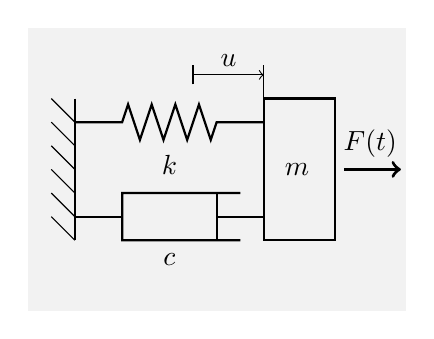
\begin{tikzpicture}[scale=0.6]
\fill[black!5!white] (-1,-3) rectangle (7, 3); 
\draw (0, 0) pic [scale=0.6] {DKbase};
\draw (0, 1) pic [scale=0.6, thick] {DKspring=4};
\draw (0,-1) pic [scale=0.6, thick] {DKdashpot=4};  
\draw[->] (2.5, 2) --(4, 2);
\draw (2.5,1.8) -- (2.5, 2.2);
\draw[thin] (4,1.5)--(4,2.2);
\draw[thick] (4,-1.5) rectangle +(1.5, 3); 
\draw (2.0, 0.1) node {$k$};
\draw (2.0,-1.9) node {$c$};
\draw (4.7, 0) node {$m$};
\draw (3.25, 2.3) node {$u$};
\draw[->, very thick] (5.7, 0) -- (6.9, 0);
\draw (6.25, 0.55) node {$F(t)$};
\end{tikzpicture}

\only<1>{\hfill 
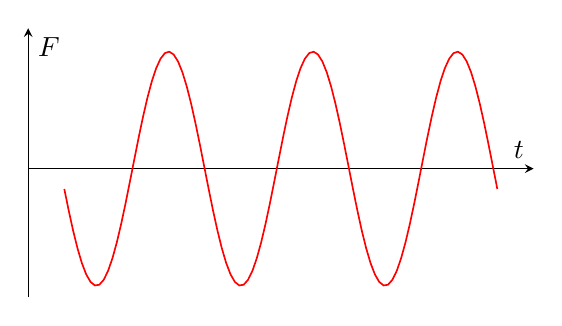
\begin{tikzpicture}
\begin{axis}[
    width=8cm, 
    height=5cm,
    axis x line=center, 
    axis y line=middle, 
    xlabel={$t$},
    ylabel={$F$},
    samples=100,
    ymin=-1.1, ymax=1.2,
    xmin=0, xmax=11,
    domain=0.25*pi:3.25*pi,
    ticks=none
]
\addplot [mark=none, semithick, red] {cos(2*deg(x)+10)};
\end{axis}
\end{tikzpicture}

}
\only<2>{\hfill 
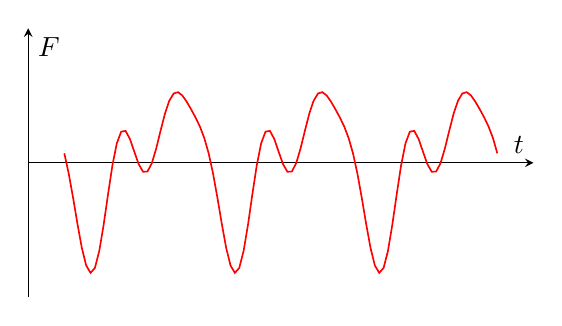
\begin{tikzpicture}
\begin{axis}[
    width=8cm, 
    height=5cm,
    axis x line=center, 
    axis y line=middle, 
    xlabel={$t$},
    ylabel={$F$},
    samples=100,
    ymin=-2, ymax=2,
    xmin=0, xmax=11,
    domain=0.25*pi:3.25*pi,
    ticks=none
]
\addplot [mark=none, semithick, red] {0.9*cos(2*deg(x)+10)-0.6*cos(4*deg(x)+80)+0.3*cos(6*deg(x)+40)};
\end{axis}
\end{tikzpicture}

}

\begin{itemize}[<+->]
 \item harmonische Anregung $F(t)=  F_C\cos\omega t + F_S\sin\omega t$ {\Large \color{green}\checkmark}
 \item allgemeine periodische Anregung $F(t+T)=F(t)$ \dots
\end{itemize}
\end{frame}

\begin{frame}
\frametitle{Vorgehensweise \normalsize{(nur für lineare Systeme)}}

\only<1>{
\begin{center}
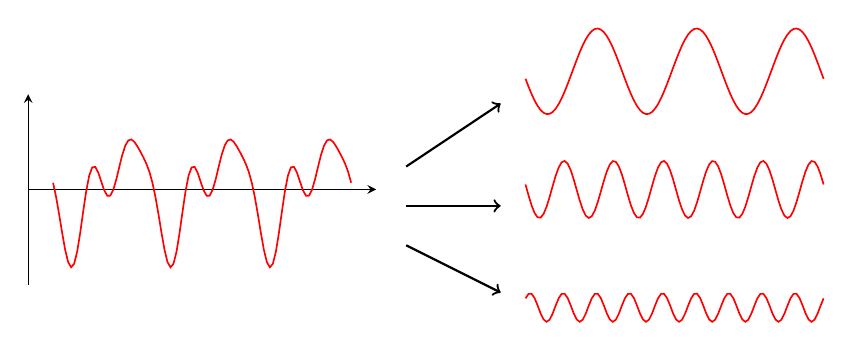
\begin{tikzpicture}
\begin{axis}[
    width=6cm, 
    height=4cm,
    axis x line=center, 
    axis y line=middle, 
    samples=100,
    ymin=-2, ymax=2,
    xmin=0, xmax=11,
    domain=0.25*pi:3.25*pi,
    ticks=none
]
\addplot [mark=none, semithick, red] {0.9*cos(2*deg(x)+10)-0.6*cos(4*deg(x)+80)+0.3*cos(6*deg(x)+40)};
\end{axis}
\begin{axis}[at={(6cm,1.5cm)},hide axis,
    width=6cm, 
    height=4cm,
    samples=100,
    ymin=-2, ymax=2,
    xmin=0, xmax=11,
    domain=0.25*pi:3.25*pi,
    ticks=none
]
\addplot [mark=none, semithick, red] {0.9*cos(2*deg(x)+10)};
\end{axis}
\begin{axis}[at={(6cm,0cm)},hide axis,
    width=6cm, 
    height=4cm,
    samples=100,
    ymin=-2, ymax=2,
    xmin=0, xmax=11,
    domain=0.25*pi:3.25*pi,
    ticks=none
]
\addplot [mark=none, semithick, red] {-0.6*cos(4*deg(x)+80)};
\end{axis}
\begin{axis}[at={(6cm,-1.5cm)},hide axis,
    width=6cm, 
    height=4cm,
    samples=100,
    ymin=-2, ymax=2,
    xmin=0, xmax=11,
    domain=0.25*pi:3.25*pi,
    ticks=none
]
\addplot [mark=none, semithick, red] {0.3*cos(6*deg(x)+40)};
\end{axis}
\draw[->, thick] (4.8, 1.5)--(6, 2.3);
\draw[->, thick] (4.8, 1.0)--(6, 1.0);
\draw[->, thick] (4.8, 0.5)--(6, -0.1);
\end{tikzpicture}


1. Schritt: Eingangssignal (Anregung) zerlegen
\end{center}
}

\only<2>{
\begin{center}
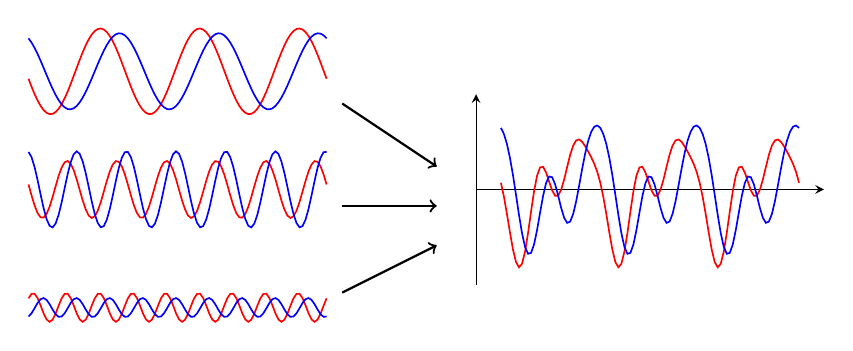
\begin{tikzpicture}
\begin{axis}[at={(0cm,1.5cm)},hide axis,
    width=6cm, 
    height=4cm,
    samples=100,
    ymin=-2, ymax=2,
    xmin=0, xmax=11,
    domain=0.25*pi:3.25*pi,
    ticks=none
]
\addplot [mark=none, semithick, red] {0.9*cos(2*deg(x)+10)};
\addplot [mark=none, semithick, blue] {0.8*cos(2*deg(x)-60)};
\end{axis}
\begin{axis}[at={(0cm,0cm)},hide axis,
    width=6cm, 
    height=4cm,
    samples=100,
    ymin=-2, ymax=2,
    xmin=0, xmax=11,
    domain=0.25*pi:3.25*pi,
    ticks=none
]
\addplot [mark=none, semithick, red] {-0.6*cos(4*deg(x)+80)};
\addplot [mark=none, semithick, blue] {-0.8*cos(4*deg(x)+10)};
\end{axis}
\begin{axis}[at={(0cm,-1.5cm)},hide axis,
    width=6cm, 
    height=4cm,
    samples=100,
    ymin=-2, ymax=2,
    xmin=0, xmax=11,
    domain=0.25*pi:3.25*pi,
    ticks=none
]
\addplot [mark=none, semithick, red] {0.3*cos(6*deg(x)+40)};
\addplot [mark=none, semithick, blue] {0.2*cos(6*deg(x)-70)};
\end{axis}
\draw[->, thick] (4.3, 2.3)--(5.5, 1.5);
\draw[->, thick] (4.3, 1.0)--(5.5, 1.0);
\draw[->, thick] (4.3,-0.1)--(5.5, 0.5);

\begin{axis}[at={(6cm, 0)}, 
    width=6cm, 
    height=4cm,
    axis x line=center, 
    axis y line=middle, 
    samples=100,
    ymin=-2, ymax=2,
    xmin=0, xmax=11,
    domain=0.25*pi:3.25*pi,
    ticks=none
]
\addplot [mark=none, semithick, red] {0.9*cos(2*deg(x)+10)-0.6*cos(4*deg(x)+80)+0.3*cos(6*deg(x)+40)};
\addplot [mark=none, semithick, blue] {0.8*cos(2*deg(x)-60)-0.8*cos(4*deg(x)+10)+0.2*cos(6*deg(x)-70)};
\end{axis}
\end{tikzpicture}


2. Schritt: Teilprobleme lösen und deren Ausgangssignale (Antwort) addieren
\end{center}

}

\end{frame}

\subsection{Fourierreihe}

\begin{frame}
\frametitle{Signalanalyse} 

\begin{figure}
   \setlength{\figW}{6.5cm} 
   \setlength{\figH}{5.2cm}
   % This file was created by tikzplotlib v0.9.4.
\begin{tikzpicture}

\begin{groupplot}[group style={group size=2 by 1}]
\nextgroupplot[
axis background/.style={fill=white!89.8039215686275!black},
axis line style={white},
height=\figH,
tick align=outside,
tick pos=left,
width=\figW,
x grid style={white},
xlabel={\(\displaystyle t\)},
xmajorgrids,
xmin=-0.0061875, xmax=0.1299375,
xtick style={color=white!33.3333333333333!black},
y grid style={white},
ylabel={\(\displaystyle y\)},
ymajorgrids,
ymin=-2.0930040296899, ymax=2.07120248233864,
ytick style={color=white!33.3333333333333!black}
]
\addplot [semithick, red]
table {%
0 0.192591610444938
0.00125 0.755262682465868
0.0025 1.49056365647655
0.00375 1.58823751078092
0.005 1.55995243628949
0.00625 1.32970259667965
0.0075 0.696146921657718
0.00875 0.351889966392085
0.01 -0.0434596669023034
0.01125 -0.104334766704289
0.0125 -0.126382264224061
0.01375 -0.0287256308594483
0.015 0.0900440761569278
0.01625 -0.115789042766529
0.0175 -0.633136390769557
0.01875 -1.13067537102531
0.02 -1.67425572395962
0.02125 -1.90372191550678
0.0225 -1.29478450457305
0.02375 -0.820606297969988
0.025 -0.0665749847635508
0.02625 1.03383824835101
0.0275 1.56082861866207
0.02875 1.88192036815552
0.03 1.56609391588191
0.03125 1.43069478825255
0.0325 0.684173789628848
0.03375 0.123386755378963
0.035 -0.22937126615034
0.03625 0.109349673615772
0.0375 0.1707218237778
0.03875 0.0720395558076415
0.04 0.0930209198493792
0.04125 -0.268096974453144
0.0425 -0.465500863503691
0.04375 -1.34098866643639
0.045 -1.60574023396326
0.04625 -1.64789864480423
0.0475 -1.4466198672644
0.04875 -0.884939210098312
0.05 0.00578659377374428
0.05125 1.04821251911132
0.0525 1.57545759655795
0.05375 1.70730308415731
0.055 1.7243487455262
0.05625 1.17634051035321
0.0575 0.457835473187691
0.05875 -0.00269543965439378
0.06 -0.188782604188503
0.06125 -0.104829820280251
0.0625 -0.0372070173478652
0.06375 0.182857878102993
0.065 -0.0528295607852067
0.06625 -0.13461733456417
0.0675 -0.673706480176667
0.06875 -1.12174473513487
0.07 -1.48617328565882
0.07125 -1.83628134422
0.0725 -1.42658605550472
0.07375 -0.881057566593151
0.075 0.0981331005080485
0.07625 0.799104721347298
0.0775 1.54116983212916
0.07875 1.87320418258098
0.08 1.63449166972165
0.08125 1.21197318898392
0.0825 0.708582329576882
0.08375 0.194704102333437
0.085 -0.0534943120684734
0.08625 0.0294594353510166
0.0875 -0.0199759908607682
0.08875 0.057425763072553
0.09 0.196421462359232
0.09125 -0.306585107863187
0.0925 -0.746708315809504
0.09375 -1.25102855367204
0.095 -1.63541539758218
0.09625 -1.72725267162278
0.0975 -1.38771571468349
0.09875 -0.848116317930947
0.1 -0.14983828462849
0.10125 0.972931009320124
0.1025 1.48710349613292
0.10375 1.88170537673295
0.105 1.6122175881445
0.10625 1.30461628444097
0.1075 0.683036786431329
0.10875 0.240534993495148
0.11 -0.107956975281847
0.11125 -0.0881342989624603
0.1125 -0.0343172382733816
0.11375 0.157357129108582
0.115 0.00576596669926299
0.11625 -0.197538419697346
0.1175 -0.779781722074558
0.11875 -1.20410848652759
0.12 -1.69057272923827
0.12125 -1.80353596409584
0.1225 -1.4373013788515
0.12375 -1.06283759643855
};

\nextgroupplot[
axis background/.style={fill=white!89.8039215686275!black},
axis line style={white},
height=\figH,
tick align=outside,
tick pos=left,
width=\figW,
x grid style={white},
xlabel={\(\displaystyle f\)},
xmajorgrids,
xmin=-6.6, xmax=138.6,
xtick style={color=white!33.3333333333333!black},
y grid style={white},
ymajorgrids,
ymin=-0.0599489893962803, ymax=1.26688579641203,
ytick style={color=white!33.3333333333333!black}
]
\addplot [semithick, red]
table {%
0 0.0100868900753801
1.33333333333333 0.007832992345893
2.66666666666667 0.00690709628524375
4 0.00625957626654251
5.33333333333333 0.00337691960011699
6.66666666666667 0.00513441034775972
8 0.00412850319159056
9.33333333333333 0.00320831230856832
10.6666666666667 0.00713885823840239
12 0.00887458536386765
13.3333333333333 0.00273624167588584
14.6666666666667 0.00496675371892951
16 0.009019686428796
17.3333333333333 0.00104144611547101
18.6666666666667 0.0013688463589634
20 0.00659964944238011
21.3333333333333 0.010551131191463
22.6666666666667 0.0061741072568213
24 0.00838063994807147
25.3333333333333 0.00282999868542395
26.6666666666667 0.00556446319492516
28 0.00967825317450989
29.3333333333333 0.00743484114965473
30.6666666666667 0.00346492100085881
32 0.00421549697371037
33.3333333333333 0.00470465237073452
34.6666666666667 0.0105485689528717
36 0.00309555650839143
37.3333333333333 0.014362897626273
38.6666666666667 0.00754066056177085
40 1.20657512432983
41.3333333333333 0.0115700474887432
42.6666666666667 0.00828726264774167
44 0.00149752021549804
45.3333333333333 0.00496734178978335
46.6666666666667 0.00445590218639584
48 0.00229737385827064
49.3333333333333 0.0104577993706734
50.6666666666667 0.0133073082265849
52 0.00575925859596791
53.3333333333333 0.00335536696962644
54.6666666666667 0.00550227264624837
56 0.00772318605625677
57.3333333333333 0.00614956687246872
58.6666666666667 0.00671253827227859
60 0.0108021406464957
61.3333333333333 0.00699424243615567
62.6666666666667 0.00841956822127757
64 0.000361682685915396
65.3333333333333 0.00356570528530283
66.6666666666667 0.00321929510782719
68 0.00798138649779375
69.3333333333333 0.00652122980520421
70.6666666666667 0.00371536471339086
72 0.00456876325941146
73.3333333333333 0.0148346237218537
74.6666666666667 0.00712923141813682
76 0.00174088206462337
77.3333333333333 0.00353748524059504
78.6666666666667 0.00989782509758069
80 0.822044783820828
81.3333333333333 0.00791335366213643
82.6666666666667 0.0066289996566685
84 0.00261858966210706
85.3333333333333 0.00361262462602836
86.6666666666667 0.00812622128875038
88 0.00593257018843588
89.3333333333333 0.00944016861177674
90.6666666666667 0.0047301845606215
92 0.0133177444761035
93.3333333333333 0.00460359225307075
94.6666666666667 0.006245526300824
96 0.00609995788707157
97.3333333333333 0.00838938378199634
98.6666666666667 0.0106648910539633
100 0.00991883062798738
101.333333333333 0.00318919495379854
102.666666666667 0.00228249298423653
104 0.00446824693522203
105.333333333333 0.00913026030743328
106.666666666667 0.00937849794666382
108 0.0103242122359087
109.333333333333 0.00230626644741817
110.666666666667 0.00312953649415611
112 0.00349632263025302
113.333333333333 0.0172486271151519
114.666666666667 0.00820134775001903
116 0.0107104181369242
117.333333333333 0.00955564531504047
118.666666666667 0.00897983449774487
120 0.00368808913543042
121.333333333333 0.00354153503067694
122.666666666667 0.0106648127500298
124 0.0084046538817176
125.333333333333 0.00579532308859913
126.666666666667 0.00849429782500491
128 0.00770301143148158
129.333333333333 0.00427365043658133
130.666666666667 0.00272057230723421
132 0.00363591297991636
};
\end{groupplot}

\end{tikzpicture}

\caption*{Leicht verrauschter Zeitverlauf und dessen Spektrum (FFT)}
\end{figure}

\begin{tabular}{ll}
Anmerkung: & Oft wird vor der FFT eine \textsl{Fensterung} angewandt,  \\
 & um Diskretisierungseffekte zu kompensieren (Kompromiss).\\
\end{tabular}

\end{frame}



\begin{frame}
\frametitle{Darstellungsarten {\normalsize -- diskrete Signale}}
Die Grundidee demonstrieren wir an einem diskreten Signal $\mathbf{s}$.

\vfill

\begin{columns}
        \begin{column}[t]{.35\linewidth}
        \only<1>{
\begin{tikzpicture}
 \draw[->] (-0.5, 0) -- (4, 0);
 \draw[->] (0,-0.5) -- (0, 4);
 \draw[dashed] (1, 2.75) -- (2, 3) -- (3, 3.5);
 \draw[fill] (1, 2.75) circle [radius=0.1];
 \draw[fill] (2, 3) circle [radius=0.1];
 \draw[fill] (3, 3.5) circle [radius=0.1];
 \draw[fill, red] (1, 1) circle [radius=0.1];
 \draw[red] (1, 0) -- (1, 1);
 \draw[fill, green] (2, 1) circle [radius=0.1];
 \draw[green] (2, 0) -- (2, 1);
 \draw[fill, blue] (3, 1) circle [radius=0.1];
 \draw[blue] (3, 0) -- (3, 1);
\end{tikzpicture}

         }
         \only<2-3>{
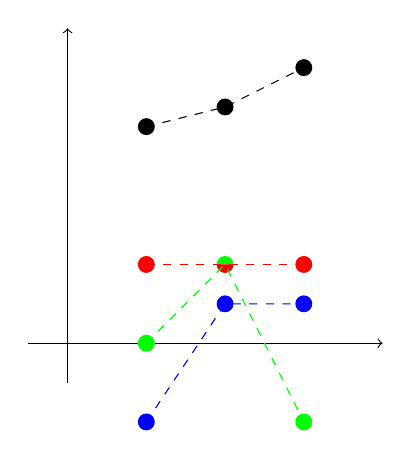
\begin{tikzpicture}
 \draw[->] (-0.5, 0) -- (4, 0);
 \draw[->] (0,-0.5) -- (0, 4);
 \draw[dashed] (1, 2.75) -- (2, 3) -- (3, 3.5);
 \draw[fill] (1, 2.75) circle [radius=0.1];
 \draw[fill] (2, 3) circle [radius=0.1];
 \draw[fill] (3, 3.5) circle [radius=0.1];
 \draw[fill, red] (1, 1) circle [radius=0.1];
 \draw[fill, red] (3, 1) circle [radius=0.1];
 \draw[dashed, red] (1,1) -- (2,1) -- (3,1);
 \draw[fill, green] (2.1,1) arc [start angle=0, end angle=180, radius=0.1];
 \draw[fill, red] (1.9,1) arc [start angle=180, end angle=360, radius=0.1];
 \draw[fill, green] (1, 0) circle [radius=0.1];
 \draw[fill, green] (3,-1) circle [radius=0.1];
 \draw[dashed, green] (1,0) -- (2,1) -- (3,-1);
 \draw[fill, blue] (1,-1) circle [radius=0.1];
 \draw[fill, blue] (2, 0.5) circle [radius=0.1];
 \draw[fill, blue] (3, 0.5) circle [radius=0.1];
 \draw[dashed, blue] (1,-1) -- (2, 0.5) -- (3, 0.5);
 \end{tikzpicture}
         
         }
        \end{column}
		\hfill
		\begin{column}[t]{.65\linewidth}
		\only<1>{\vspace{1cm}
		
         $\mathbf{s}=a_1\mathbf{b}_1 + a_2\mathbf{b}_2 + a_3\mathbf{b}_3$ \\[1cm]
{\color{red} $\mathbf{b}_1=\left[\begin{array}{c} 1\\ 0\\ 0 \end{array}\right]$}, \quad
{\color{green} $\mathbf{b}_2=\left[\begin{array}{c} 0\\ 1\\ 0 \end{array}\right]$}, \quad
{\color{blue} $\mathbf{b}_3=\left[\begin{array}{c} 0\\ 0\\ 1 \end{array}\right]$}.        
         }
         \only<2-3>{\vspace{1cm}
         
                  $\mathbf{s}=a_1\mathbf{b}_1 + a_2\mathbf{b}_2 + a_3\mathbf{b}_3$ \\[1cm]
{\color{red} $\mathbf{b}_1=\left[\begin{array}{c} 1\\ 1\\ 1 \end{array}\right]$}, \quad
{\color{green} $\mathbf{b}_2=\left[\begin{array}{c} 0\\ 1\\ -1 \end{array}\right]$}, \quad
{\color{blue} $\mathbf{b}_3=\left[\begin{array}{c} -1\\ 1/2\\ 1/2 \end{array}\right]$}.        
         }
		\end{column}
\end{columns}

\vfill
\only<3>{ \alert{\textbf{HA}: Zeigen Sie die lineare Unabhängigkeit beider Darstellungen.}}\end{frame}

\begin{frame}
\frametitle{Darstellungsarten {\normalsize -- kontinuierliche Signale}}
Im Grenzübergang (unendlich viele Punkte) lassen sich stetige Funktionen punktweise oder als Summe (unendlich vieler) Basisfunktionen darstellen.

\bigskip

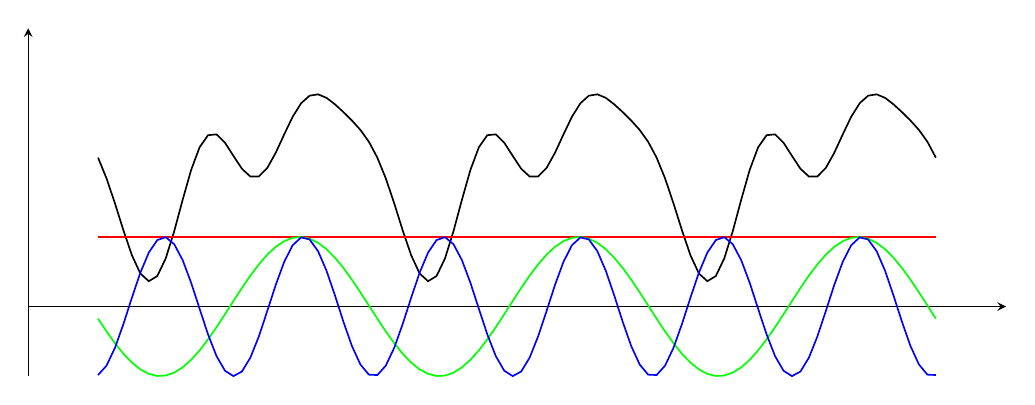
\begin{tikzpicture}
\begin{axis}[
    width=14cm, 
    height=6cm,
    axis x line=center, 
    axis y line=middle, 
    samples=100,
    ymin=-1, ymax=4,
    xmin=0, xmax=11,
    domain=0.25*pi:3.25*pi,
    ticks=none
]
\addplot [semithick] {2+0.9*cos(2*deg(x)+10)-0.6*cos(4*deg(x)+80)+0.3*cos(6*deg(x)+40)};
\addplot [semithick, red] {1};
\addplot [semithick, green] {cos(2*deg(x)+10)};
\addplot [semithick, blue] {cos(4*deg(x)+10)};
\end{axis}
\end{tikzpicture}


\bigskip

Im Fall der Fourierreihe stellen trigonometrische Funktionen die Basis dar.
\end{frame}

\begin{frame}
\frametitle{Exkurs -- Orthogonalität}
Zwei Vektoren $\mathbf{v}_1$ und $\mathbf{v}_2$ sind orthogonal, 
wenn ihr Skalarprodukt verschwindet
\begin{equation*}
\mathbf{v}_1  \cdot \mathbf{v}_2 =0 .
\end{equation*}
Die Verallgemeinerung auf Funktionen lautet
\begin{equation*}
\int_{a}^{b} \mathbf{f}_1(x)\,\mathbf{f}_2(x)\,\mathrm{d}x =0 .
\end{equation*}
Die Funktionen der Fourierrreihe ($m,n \in \mathbb{N}$) sind orthogonal zueinander
\begin{align*}
\int_{0}^{2\pi} \cos mx\, \sin nx\,\mathrm{d}x &=0,\\
\int_{0}^{2\pi} \sin mx\, \sin nx\,\mathrm{d}x=\int_{0}^{2\pi} \cos mx\, \cos nx\,\mathrm{d}x &=
\left\{\begin{array}{ll}
\pi & \text{für } m=n,\\
0 & \text{sonst}.
\end{array}
 \right.
\end{align*}
\end{frame}

\begin{frame}
\frametitle{Fourierreihe 1/2}
Aus den bisherigen Überlegungen wissen wir, dass sich periodische Funktionen $g(\theta+2\pi)=g(\theta)$ folgendermaßen darstellen lassen
\begin{equation*}
 g(\theta)=\frac{1}{2}A_0 + \sum_{k=1}^{\infty} A_k \cos k\theta + B_k \sin k\theta.
\end{equation*}
Um die Koeffizienten $A_k$ und $B_k$ zu finden, 
nutzen wir die Orthogonalität der Basisfunktionen
\begin{align*}
\int_{-\pi}^{+\pi} g(\theta) \cos n\theta\,\mathrm{d}\theta 
&=\int_{-\pi}^{+\pi} \left(\frac{1}{2}A_0 + \sum_{k=1}^{\infty} A_k \cos k\theta + B_k \sin k\theta\right)  \cos n\theta \,\mathrm{d}\theta \\
&= A_n \pi,\\
\int_{-\pi}^{+\pi} g(\theta) \sin n\theta\,\mathrm{d}\theta 
&=\ \dots \ =B_n \pi.
\end{align*} 

\end{frame}

\begin{frame}
\frametitle{Fourierreihe 2/2}
Für Funktionen mit allgemeiner Periode $f(x)=f(x+\overbrace{2\pi l}^{T})$ erhalten wir ($\theta=x/l$) die Darstellung
\begin{equation*}
 f(x)=\frac{1}{2}A_0 + \sum_{k=1}^{\infty} A_k \cos(kx/l) + B_k \sin(kx/l),
\end{equation*}
mit den Koeffizienten
\begin{align*}
 A_k &=\frac{1}{\pi l}\int_{-\pi l}^{+\pi l} f(t)\cos(kt/l)\,\mathrm{d}t
     &=\frac{2}{T}\int_{-T/2}^{+T/2} f(t)\cos(2\pi kt/T)\,\mathrm{d}t
 ,\\
 B_k &=\frac{1}{\pi l}\int_{-\pi l}^{+\pi l} f(t)\sin(kt/l)\,\mathrm{d}t
     &=\frac{2}{T}\int_{-T/2}^{+T/2} f(t)\sin(2\pi kt/T)\,\mathrm{d}t.
\end{align*}


\end{frame}


\begin{frame}
\frametitle{Beispiel 1/2}

Rechtecksignal $a(t)=\left\{\begin{array}{ll}
                             1, & 0 < t \le T/2\\
                             0, & T/2 < t \le T\\
                             \,\vdots & \ \vdots 
                            \end{array}
  \right.$ 
  \hfill
  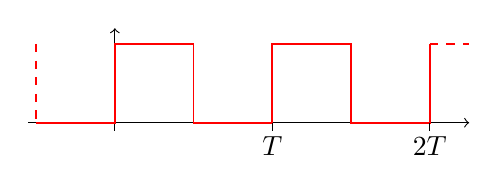
\begin{tikzpicture}[baseline=3mm] 
 \draw[->] (-1.1, 0) -- (4.5, 0);
 \draw[->] (0,-0.1) -- (0, 1.2);
 \draw[semithick,red] 
 (-1,0)-- ++(1,0)-- ++(0,1)-- ++(1,0)-- ++(0,-1)-- ++(1,0)--
 ++(0,1)-- ++(1,0)-- ++(0,-1)-- ++(1,0)-- ++(0,1);
 \draw[semithick,red, dashed] (4,1) -- (4.5,1);
 \draw[semithick,red, dashed] (-1,1) -- (-1,0); 
 \draw (2,0) -- (2,-0.1);
 \draw (4,0) -- (4,-0.1);
 \draw (2,-0.3) node {$T$};
 \draw (4,-0.3) node {$2T$};
 \end{tikzpicture}

 \begin{align*}
 A_0&=&\frac{2}{T} \int_{0}^\frac{T}{2} 1\,\mathrm{d}t&=&\frac{2}{T}\bigl|t\bigr|_{0}^{T/2}&=1, \\[1mm]
 A_k&=& \frac{2}{T} \int_{0}^\frac{T}{2} \cos\left(\frac{2\pi kt}{T}\right) \,\mathrm{d}t  
 &=&\frac{2}{T} \left|\frac{T}{2\pi k} \sin\left(\frac{2\pi kt}{T}\right) \right|_0^{T/2} &=0, \ k>0,
 \\[1mm]
 B_k&=& \frac{2}{T} \int_{0}^\frac{T}{2} \sin\left(\frac{2\pi kt}{T}\right) \,\mathrm{d}t  
 &=&\frac{2}{T} \left|\frac{-T}{2\pi k} \cos\left(\frac{2\pi kt}{T}\right) \right|_0^{T/2} &=
 \left\{\begin{array}{ll}
    \frac{2}{\pi k},& k=1,3, \dots ,\\
    0, & k=2,4, \dots .
        \end{array} \right.
 \end{align*}
 
\end{frame}


\begin{frame}
\frametitle{Beispiel 2/2}
\begin{figure}
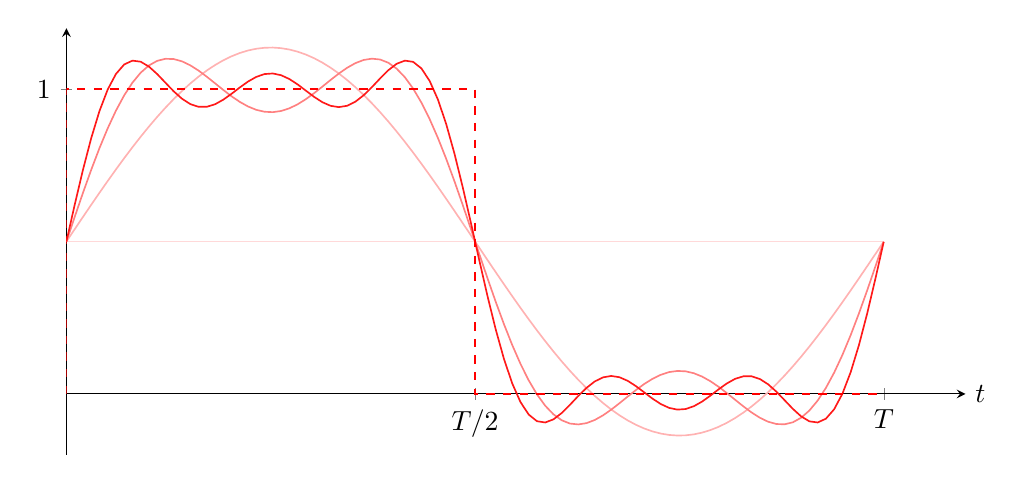
\begin{tikzpicture}
\begin{axis}[
    width=13cm, 
    height=7cm,
    axis x line=center, 
    axis y line=middle, 
    xlabel={$t$},
     x label style={at={(current axis.right of origin)}, right},
    samples=100,
    ymin=-0.2, ymax=1.2,
    xmin= 0, xmax=1.1,
    domain=0:1,
    xtick={   0.5,  1  },
    xticklabels={ $T/2$ , $T$ }, 
    ytick={0, 1},
    yticklabels={$0$, $1$}
]
\addplot [mark=none, semithick, red!15!white] {0.5};   %sin(deg(x))
\addplot [mark=none, semithick, red!30!white] {0.5+(2/pi)*sin(deg(2*pi*x))};   
\addplot [mark=none, semithick, red!50!white] {0.5+(2/pi)*sin(deg(2*pi*x))+(2/(3*pi))*sin(deg(6*pi*x))};   
\addplot [mark=none, semithick, red!90!white] {0.5+(2/pi)*sin(deg(2*pi*x))+(2/(3*pi))*sin(deg(6*pi*x))++(2/(5*pi))*sin(deg(10*pi*x))};   %
\draw[red, dashed, semithick] (axis cs: 0, 0) -- (axis cs: 0, 1) -- (axis cs: 0.5, 1) -- (axis cs: 0.5, 0) -- (axis cs: 1, 0);
\end{axis}
\end{tikzpicture}

\caption{Approximation des Rechteckimpulses als Fourierreihe ($k=1,2,3,5$)}
\end{figure}
\end{frame}


\begin{frame}
\frametitle{Anschauliche Darstellung}
\vfill
\begin{center}

\includegraphics[width=0.2\textwidth]{fig_img/youtube.png}  

\href{https://www.youtube.com/watch?v=ds0cmAV-Yek}{\textsl{SmarterEveryDay: Was ist eine Fourierreihe?}}
\end{center}  
\vfill
\end{frame}




\subsection{Allgemeine periodische Anregung}

\begin{frame}
\frametitle{Superpositionsprinzip}
\begin{center}
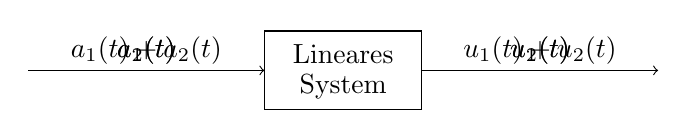
\begin{tikzpicture}
\draw (0, 0.21) node {Lineares};
\draw (0,-0.21) node {System};
\draw (-1,-0.5) rectangle (1, 0.5);
\draw[->] (-4, 0) -- (-1, 0);
\draw[->] ( 1, 0) -- ( 4, 0);
\draw[visible on=<1>] (-2.5, 0.25) node {$a_1(t)$};
\draw[visible on=<1>] ( 2.5, 0.25) node {$u_1(t)$};
\draw[visible on=<2>] (-2.5, 0.25) node {$a_2(t)$};
\draw[visible on=<2>] ( 2.5, 0.25) node {$u_2(t)$};
\draw[visible on=<3->] (-2.5, 0.25) node {$a_1(t)+a_2(t)$};
\draw[visible on=<3->] ( 2.5, 0.25) node {$u_1(t)+u_2(t)$};
\end{tikzpicture}

\end{center}
\uncover<3>{
Vorgehen für den (allgemein) periodisch erregten Einmassenschwinger 
\begin{align*}
a(t)&=\frac{1}{2}A_0 + \sum_{k=1}^{\infty} A_k \cos\left(\frac{2\pi kt}{T}\right) + B_k\left(\frac{2\pi kt}{T}\right)\\
&\approx\frac{1}{2}A_0 + \sum_{k=1}^{N} A_k \cos\left(\frac{2\pi kt}{T}\right) + B_k\left(\frac{2\pi kt}{T}\right)\\
u(t)&= \sum_{k=1}^{\infty} u_k(t) \approx \sum_{k=1}^{N} u_k(t)
\end{align*}
}
\end{frame}


\begin{frame}
\frametitle{Anwendungsbeispiel}
\begin{figure}
 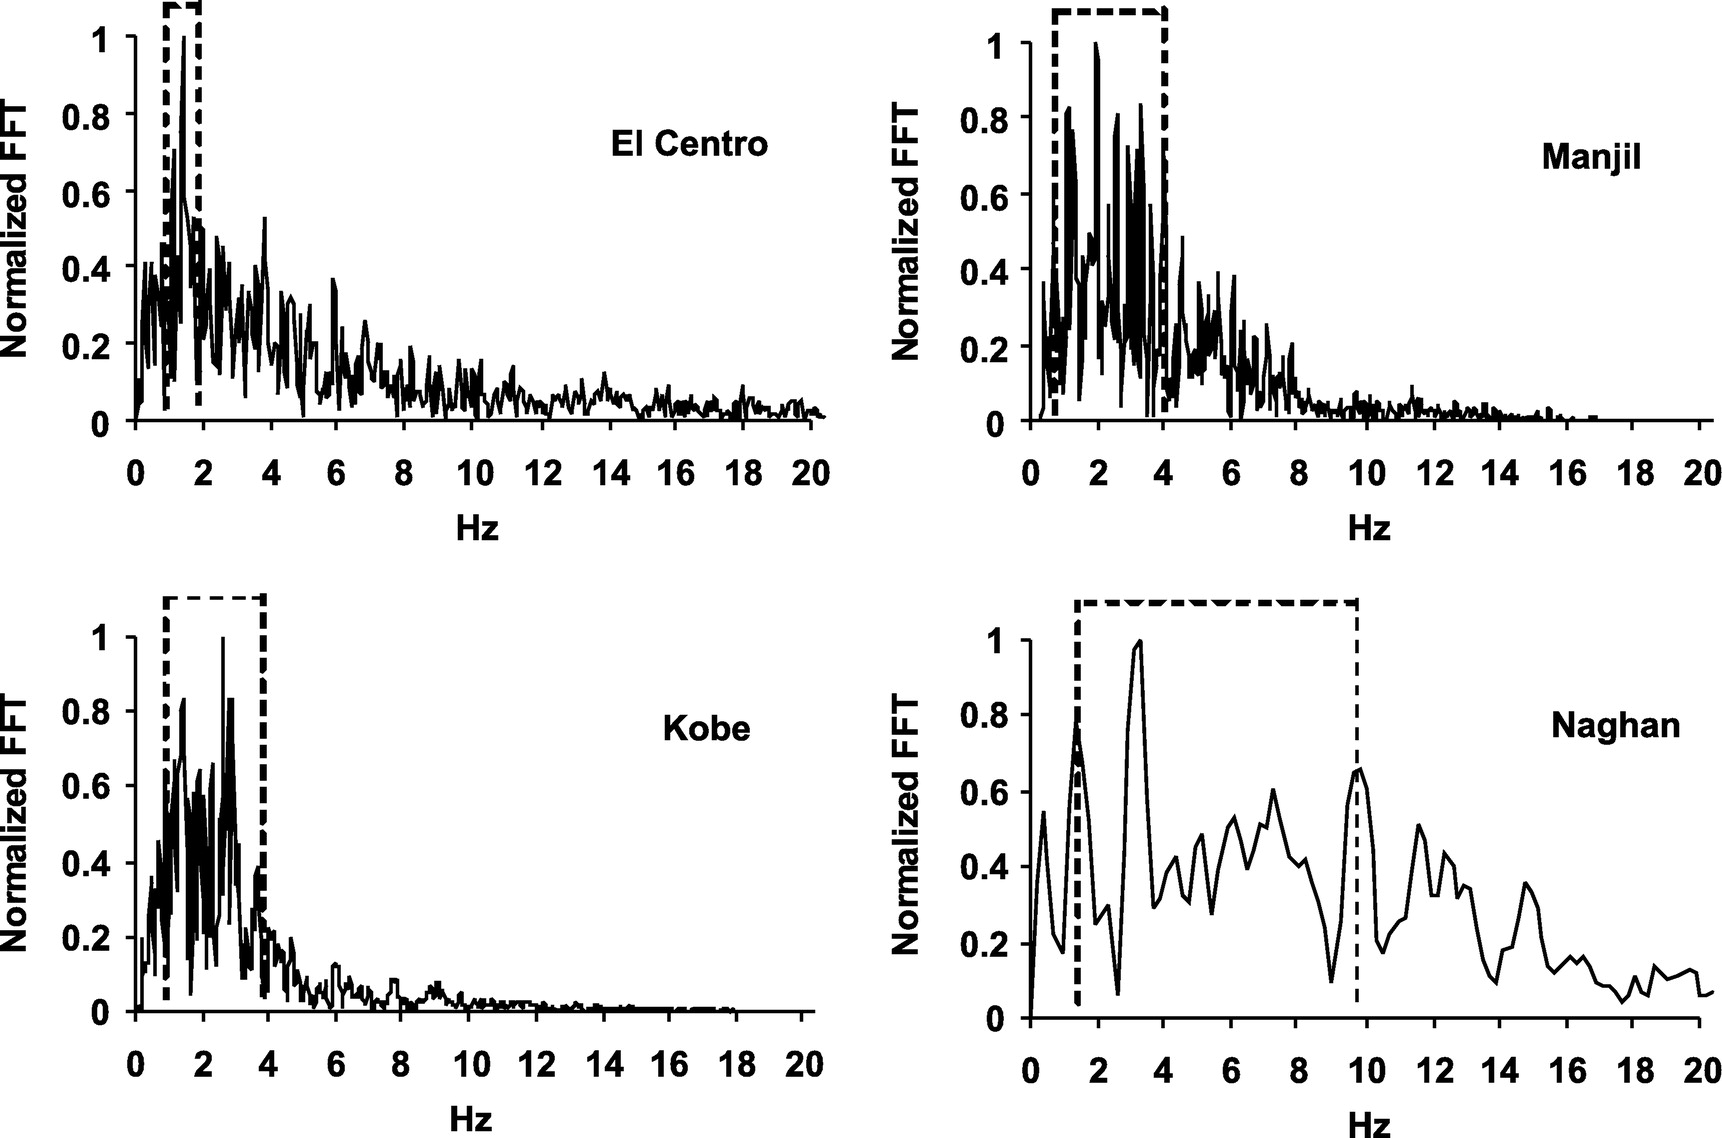
\includegraphics[width=0.7\textwidth]{fig_img/earthquake_spectra.jpg}
 \caption*{Amplitudenspektrum ausgewählter Erdbeben \cite{amiri2008}}
\end{figure}
Anmerkung: Dieses Vorgehen wäre für Überschlagsrechnungen angebracht.

\end{frame}



\begin{frame}
\frametitle{Zusatzmaterial} % physical intution and complex representation
\vfill
\begin{center}

\includegraphics[width=0.2\textwidth]{fig_img/youtube.png}  

\href{https://www.youtube.com/watch?v=spUNpyF58BY}{\textsl{3Blue1Brown: Was ist eine Fourier-Transformation?}}
\end{center}  
\vfill
\end{frame}


%%%%%%%%%%%%%%%%%%%%%%%%%%%%%%%%%%%%%%%%%%%%%%%%

\section*{Literaturverzeichnis}

\begin{frame}[allowframebreaks]{}
	\printbibliography
\end{frame}


\end{document}
